%   SETUP%
\documentclass[a4paper,11pt,oneside,titlepage]{book}
\usepackage[T1]{fontenc}		% Codifica dei font; T1 codifica di output dell'italiano e di lingue occidentali
\usepackage[utf8]{inputenc}		% Codifica degli input; abilita l'utilizzo di caratteri accentati
\usepackage[italian]{babel}		% Set the languages; the last one is the main language
\usepackage{geometry}			% Allow to change the margin
\usepackage{setspace}			% Allow to change the interline with \begin{onehalfspaceng} ecc.
\usepackage{fancyhdr}			% Fancy style for page layout
\usepackage{afterpage} 			% Allow to load blank pages with the command '\afterpage{\null\thispagestyle{empty}\clearpage}' 
\usepackage{hyperref}			% Crea collegamenti ipertestuali rendendo cliccabili i riferimenti
\usepackage{url}
\usepackage{color}			% Allow to use colors
\usepackage{xcolor}			% manage colors
\usepackage{enumerate}			% Numbered lists
\usepackage{enumitem}			% Allow to manage the style of the list
\usepackage{graphicx}			% Images
\usepackage{epstopdf}			% allows to convert eps images to pdf for use with pdflatex
\usepackage{pstool}			% Allows to use psfrag with pdflatex (no latex compiler needed)
\usepackage{psfrag}
%\usepackage[normal]{subfigure}		% manage subfigures
\usepackage{subfig}		% manage subfigures
\usepackage{array}			% Tables
\usepackage{tabularx}			% allow to set the width of the whole table
\usepackage[bottom]{footmisc}		% To attach footnote at the end of the page
\usepackage{booktabs}			% is a must for professional-looking layout
\usepackage{longtable}			% is very popular for multi-page tables
\usepackage{caption}			% Captions
\usepackage{float}			% Manage float objects (image, table, ecc.)
\usepackage{rotating}			% permette di ruotare immagini, tabelle, ecc. di 90° o di 270°
\usepackage{rotfloat}			% costruisce un ponte tra i pacchetti float e rotating
\usepackage{amsmath} 			% Equations
\usepackage{amssymb}			% Mathematical Symbols
\usepackage{cancel}                     % Simplification Cancellation
\usepackage{mleftright}
\usepackage{listings}                   % Codes
\definecolor{lstgreen}{rgb}{0,0.6,0}
\definecolor{lstgray}{rgb}{0.5,0.5,0.5}
\definecolor{lstmauve}{rgb}{0.58,0,0.82}
\lstset{ %
  backgroundcolor=\color{white},   % choose the background color
  basicstyle=\footnotesize,        % size of fonts used for the code
  breaklines=true,                 % automatic line breaking only at whitespace
  captionpos=b,                    % sets the caption-position to bottom
  commentstyle=\color{lstgreen},    % comment style
  escapeinside={\%*}{*)},          % if you want to add LaTeX within your code
  keywordstyle=\color{blue},       % keyword style
  stringstyle=\color{lstmauve},     % string literal style
}
%\usepackage{vector}  			% Allows "\bvec{}" and "\buvec{}" for "blackboard" style bold vectors in maths
\usepackage[swapnames,norules,nouppercase]{frontespizio}
\usepackage[intoc]{nomencl}
\usepackage[acronym,toc,nomain,nopostdot,nonumberlist]{glossaries}
\usepackage[square, numbers, comma, sort&compress]{natbib}
\usepackage{verbatim}                   % Needed for the "comment" environment to make LaTeX comments
\usepackage{wrapfig}                 % Per inserire le figure contornate da testo
\usepackage{blindtext}
\geometry{a4paper,top=2.5cm,bottom=2.5cm,left=2cm,right=2cm,heightrounded,bindingoffset=5mm,headheight=13.6pt}
% -------------------------------------- Line-spacing --------------------------------------- %
\linespread{1.2} 
%\linespread{1.5} 
%\linespread{2} 
%\raggedbottom % disattiva lo 'stiracchiamento' del testo; va a favore di spazio bianco a fondo pagina
% ---------------------------------------- Numeration --------------------------------------- %
%\setcounter{secnumdepth}{3} % set the enumeration of the sections
%\setcounter{tocdepth}{3}    % set the enumeration of the sections in the table of contents
%--------------------------------------- Page layout -----------------------------------------%
%\pagestyle{fancy}                       % definisce lo stile di pagina aprendo la strada al pacchetto fancyhdr
%\renewcommand{\chaptermark}[1]{\markright{\chaptername\ \thechapter.\ #1}{}}    % ridefinisce la macro \rightmark per i capitoli
%\renewcommand{\sectionmark}[1]{\markright{\sectionname\ \thesection.\ #1}}      % ridefinisce la macro \rightmark per le sezioni
%\renewcommand{\sectionmark}[1]{\markright{\thesection.\ #1}}
%\lhead{Giacomo Della Posta}             % in alto a sinistra
%\chead{}                                % in alto al centro
%\rhead{\slshape \rightmark}             % in alto a destra (\rightmark contiene ...)
%\lfoot{Giacomo Della Posta}             % in basso a sinistra
%\cfoot{\thepage}                        % in basso al centro (\thepage per mettere il numero di pagina)
%\rfoot{}                                % in basso a destra
%\renewcommand{\headrulewidth}{0.4pt}    % spessore della linea di separazione in alto (0 per eliminare la linea)
%\renewcommand{\footrulewidth}{0.4pt}    % spessore della linea di separazione in basso (0 per eliminare la linea)
\fancypagestyle{plain}{%                                        % modifica dello stile predefinito plain
                        \fancyhf{}                              % cancella tutti i campi di  intestazione e pie di pagina
                        \fancyfoot[R]{\thepage}                 % mette al centro il numero di pagina
                        \renewcommand{\headrulewidth}{0pt}      % spessore della linea di separazione in alto (0 per eliminare la linea)
                        \renewcommand{\footrulewidth}{0.4pt}    % spessore della linea di separazione in basso (0 per eliminare la linea)
                        }                                       % modifica dello stile predefinito plain
\captionsetup{font=small,labelfont=bf,textfont=normalfont,tableposition=bottom,figureposition=bottom}
%\captionsetup{font=small,labelfont=bf,textfont=bf,tableposition=bottom,figureposition=bottom}
% ---------------------------------------- Itemize ------------------------------------------ %
%\setlist[itemize]{noitemsep, topsep=0pt} %Se non vuoi i pallini degli elenchi vuoti, allora commenta queste linee      
%\renewcommand{\labelitemi}{$\circ$}	% items i with empty bullets
%\renewcommand{\labelitemii}{$\bullet$}	% items ii with black bullets
\hypersetup{colorlinks=true, linkcolor=black, citecolor=black, filecolor=black, urlcolor=black}
\definecolor{red-univaq}{RGB}{130,36,51} % example \definecolor{name}{model}{color-spec}
\definecolor{univaq}{RGB}{242,195,80} % example \definecolor{name}{model}{color-spec}
\makenomenclature % Generate the nomenclature
\makeglossaries % Generate the glossary
%\lstset{language=[90]Fortran,
%        inputpath=/home/luca/PhD/Thesis/Code,
%        basicstyle=\small\ttfamily, 
%        xleftmargin=0cm,
%        fontadjust=true,
%        keepspaces=true,
%        basewidth=0.5em,
%        breakatwhitespace=false,           % sets if automatic breaks should only happen at whitespace
%        breaklines=false,                  % sets automatic line breaking
%        captionpos=b,                     % b=bottom
%        backgroundcolor=\color{white},
%        identifierstyle=\color{black},
\bibliographystyle{abbrv} % abbrv --> [1], [2], ecc.
%\bibliographystyle{unsrtnat} 
% ---------------------------------------- Dedication ------------------------------------------ %
\newenvironment{dedication}
{
  \phantom{.}
  \vspace{13cm}
  \begin{quote} \begin{flushright}}
{\end{flushright} \end{quote}}
\usepackage{calligra}

\begin{document}

%   FRONT MATTER                                            %
\frontmatter 	   % Begin Roman style (i, ii, iii, iv...) page numbering
\pagestyle{empty}  % No headers or footers for the following pages

%   TITLE PAGE
\begin{frontespizio}
% Remember: After editing this file, delete the cache and recompile
%---------------------Definizione font---------------------%
\Preambolo{\renewcommand{\fronttitlefont}{\fontsize{24}{24}\bfseries}}
%----------------------------------------------------------%
	% \frontinstitutionfont 	Neretto, 14/17 
	% \frontdivisionfont 		Tondo, 12/16 
	% \frontpretitlefont 		Maiuscoletto, 10/12
	% \fronttitlefont 		Neretto, 17/21 
	% \frontsubtitlefont 		Tondo, 12/14
	% \frontfixednamesfont 		Tondo, 12/14 
	% \frontnamesfont 		Neretto, 12/14 
	% \frontsmallfont 		Neretto, 9/11 
	% \frontfootfont	 	Neretto, 12/14 

	% \bfseries	Grassetto
	% \itshape	Corsivo
	% \scshape	Maiuscoletto
%----------------------------------------------------------%
\Margini{4cm}{3cm}{3cm}{3cm} % Margini sinistro, in basso, destro e in alto
\Logo[4cm]{figures/logo/UnivAQ_logoA.eps}
%\Universita{L'Aquila}
\Istituzione{Dipartimento di Ingegneria e Scienze dell'Informazione e Matematica}
%\Divisione{Department of Information Engineering, Computer Science and Mathematics}	% ENG
\Divisione{Tesi di Laurea Triennale in Informatica}		% ITA
%\Dipartimento{Dipartimento di Ingegneria e Scienze dell'Informazione e Matematica}
%\Corso[Master Degree]{Ingegneria delle Telecomunicazioni}
\Scuola{}
\Titoletto{}

\Titolo{Dai Keypoint alla Conoscenza}
\Sottotitolo{Una pipeline per rendere il movimento umano interrogabile da agenti autonomi in modo esplicito, sicuro e verificabile}

\Punteggiatura{} % Modifica la punteggiatura dopo 'Candidato', 'Realatore' ecc. (vuoto per togliere)
\NCandidato{Laureando} % Sostituisce 'Candidato' con '...'
\Preambolo{\renewcommand{\frontsmallfont}[1]{\small}}
\Candidato[246965]{Rocchetti Claudio}

%\NRelatore{Thesis Advisor}{Relatori}
\NRelatore{Relatore}{Relatori}
\Relatore{Prof. Di Rocco Yuri}
%\NCorrelatore{Thesis Co-Advisor}{Relatori}
%\Rientro{1cm} % Rientro di Relatore e Candidato

\Piede{Anno Accademico 2025-2026}
\end{frontespizio}

\IfFileExists{\jobname-frn.pdf}{}{%
\immediate\write18{pdflatex \jobname-frn}} 
\clearpage

%   QUOTE (OPTIONAL)
\begin{dedication}

{\fontfamily{calligra}\selectfont
{\Huge


}
}
\end{dedication}



\newpage

%   ABSTRACT
\afterpage{\null\thispagestyle{empty}\clearpage} % Blank page
\thispagestyle{plain}			% Supress header 
\setlength{\parskip}{0pt plus 1.0pt}
\section*{Abstract}
% TODO: scrivere l'abstract.

% KEYWORDS (MAXIMUM 10 WORDS)
\vfill
Keywords: 

\thispagestyle{empty}
\mbox{}
 

%   TOC - LOF - LOT
\begin{singlespace}
 \tableofcontents 	
 \addcontentsline{toc}{chapter}{\listfigurename}
 \listoffigures
 \addcontentsline{toc}{chapter}{\listtablename}
 \listoftables
% \renewcommand{\lstlistlistingname}{List of Code}
% \addcontentsline{toc}{chapter}{\lstlistlistingname} 
% \lstlistoflistings

%   NOMENCLATURE AND ACRONYMS
 \printnomenclature
 \printglossaries
\end{singlespace}

%   MAIN MATTER
\mainmatter	  % Begin normal, numeric (1,2,3...) page numbering
\clearpage
% ------ set page style fancy with the follow 
\pagestyle{fancy} 
\renewcommand{\chaptermark}[1]{\markright{\chaptername\ \thechapter.\ #1}{}}
\renewcommand{\sectionmark}[1]{\markright{\thesection.\ #1}}
\lhead{} 
\chead{}                   
\rhead{\slshape \rightmark} 
\lfoot{Rocchetti Claudio}
\cfoot{} 
\rfoot{\thepage}          
\renewcommand{\headrulewidth}{0.4pt} 
\renewcommand{\footrulewidth}{0.4pt} 

%   CHAPTERS
\chapter{Introduzione}
\label{chap:introduzione}

\section{Il dato da solo non può rispondere alle domande}
\label{sec:ch1:contesto}

Possiamo distinguere due diversi tipi di metodo di acquisizione dei dati di posa umana. 
I sistemi di laboratorio che misurano decine di marker con metodi matematici accurati tramite sensori ad-hoc, ed i 
sistemi di cattura del movimento tramite videocamere che stimano la posizione dei punti di posa in uno spazio tridimensionale.

Entrambi però da soli non possono rispondere a domande semplici come \emph{``quanto flette il
ginocchio destro in questa sessione?''}. In questo caso, ad esempio, per poter rispondere bisognerebbe 
prima definire quali siano le coordinate del ginocchio, cosa si intenda per flessione, in quale intervallo di tempo e se i dati 
bastino a poter dare realmente una risposta. Niente di tutto ciò è scritto nel file, inoltre sistemi diversi possono avere 
nomenclature diverse. Il significato dei numeri è confinato quindi nell'infrastruttura dove il dato viene prodotto, sorge 
quindi un problema quando il destinatario della risposta è esterno.

\section{Gli agenti conversazionali ed il cambio di paradigma}
\label{sec:ch1:agenti}

Un agente conversazionale, diversamente da un umano, proverà sempre a rispondere alla domanda 
cercando di interpretare i dati, è qui che il paradigma cambia radicalmente. Prima il problema era non 
poter dare una risposta, ora è ricevere una risposta sbagliata posta in modo che sembri plausibile.

Chiedere al modello di essere prudente non basta, la garanzia va collocata nel
software che il modello interroga. È il software stesso a trasformare il dato grezzo, 
conservarlo in modo riproducibile, giudicarlo rispetto a riferimenti citabili e
a dichiarare ciò che si possa o meno affermare. Questo progetto prova a creare questo strato 
intermedio per metterlo a disposizione degli agenti.

\section{Obiettivi progettuali}
\label{sec:ch1:obiettivi}

Il lavoro si pone cinque obiettivi, a cui il resto della tesi si riferisce.

\begin{enumerate}[label=\textbf{O\arabic*.},leftmargin=*]
  \item Una pipeline che trasforma sorgenti eterogenee, cioè file di laboratorio
    e riprese da videocamera , in un unico formato 
    canonico che porta con sé provenienza, copertura ed eventuali assenze.
  \item Un archivio interrogabile composto da punti di posa scalari e cicli di movimento vettoriali, così da poter cercare gesti simili e misurare
    ripetibilità e simmetria.
  \item Un sistema di alert dichiarativo, in cui ogni soglia ha una fonte di
    letteratura e ogni avviso la riporta.
  \item Un server conforme al Model Context Protocol~\cite{mcpspec} che espone queste capacità a
    qualunque agente, con risposte che dichiarano segnale e copertura.
  \item Una visualizzazione tridimensionale per le intere sessioni che mostri, oltre al movimento del soggetto, gli scostamenti dai valori di letteratura.
\end{enumerate}

Gli angoli seguono convenzioni riconosciute e sono verificati da un confronto diretto con un modello clinico; 
il contributo del lavoro riguarda ciò che il software permette di fare
con quei dati. Non sono trattati invece il miglioramento dell'accuratezza di cattura e la validazione clinica dei valori di riferimento.

\section{Struttura della tesi}
\label{sec:ch1:struttura}

Il Capitolo~\ref{chap:background} descrive le idee ed i problemi durante la creazione della pipeline.
Il Capitolo~\ref{chap:architettura} presenta, nello stesso ordine, le soluzioni
adottate. Il Capitolo~\ref{chap:casi-uso} mostra il sistema a lavoro, con alcune
dimostrazioni e tre casi d'uso eseguiti da due agenti diversi. Il
Capitolo~\ref{chap:comparazione} descrive la differenza di questo progetto rispetto agli
strumenti esistenti. Il Capitolo~\ref{chap:discussione} raccoglie limiti e
sviluppi futuri, infine il Capitolo~\ref{chap:conclusioni} i risultati.

\chapter{Background e problem statement}
\label{chap:background}

\chapter{Approccio proposto e architettura}
\label{chap:architettura}

\chapter{Tre casi d'uso reali}
\label{chap:casi-uso}

\chapter{Differenziazione dagli strumenti esistenti}
\label{chap:comparazione}

\section{Su quali assi ci si differenzia}
\label{sec:ch5:assi}

Nessuno degli strumenti considerati prova a fare ciò che fa questo sistema, quindi
su ciascun terreno, preso da solo, il risultato del confronto è scontato. La
differenza emerge solo tenendo insieme tre assi.

\begin{enumerate}[label=\textbf{A\arabic*.},leftmargin=*]
  \item La profondità biomeccanica, ovvero quanto il sistema arriva vicino alla
    cinematica articolare e con quale modello.
  \item L'interrogabilità, ovvero quanto si possono porre domande in linguaggio
    naturale da parte di una persona o di un agente.
  \item L'onestà dichiarata, ovvero quanto il sistema comunica, insieme al
    risultato, la qualità del dato su cui si basa.
\end{enumerate}

Gli strumenti esistenti ne coprono al massimo due, mentre lo spazio in cui si
colloca questo lavoro è proprio la combinazione dei tre.

\section{Prima famiglia, chat su metriche di allenamento}
\label{sec:ch5:allenamento}

La prima famiglia comprende le piattaforme che rendono conversazionali i dati di
allenamento. Kailo\cite{kailo}, che in precedenza si chiamava GetFast, affianca all'analisi
dell'allenamento una chat rivolta all'atleta, AI Endurance\cite{aiendurance} pubblica
un server MCP ufficiale, mentre per TrainingPeaks\cite{trainingpeaksmcp} esiste un
connettore MCP non ufficiale, segno che la domanda di
integrazione con gli agenti è già presente.

L'interrogabilità è pienamente coperta ed il motivo è lo stesso che tiene queste
piattaforme lontane dalla biomeccanica articolare, perché le grandezze esposte,
come passo, cadenza e carico, sono già aggregate ed interpretate. Non esiste
quindi, ad esempio, un angolo del ginocchio da sbagliare e per la stessa ragione il problema
dell'onestà sul dato articolare non si pone. Il sistema proposto prova invece a
portare l'interrogabilità dentro il dominio articolare.

\section{Seconda famiglia, biomeccanica markerless professionale}
\label{sec:ch5:markerless}

La seconda famiglia ricostruisce la cinematica articolare da video con
un'accuratezza validata. OpenCap\cite{opencap}, sviluppato a Stanford ed open source, lo fa a
partire da due telecamere di smartphone, mentre Theia3D\cite{theia3d} è una
soluzione commerciale a corpo intero basata su video
multicamera.

Sulla profondità biomeccanica questi sistemi sono migliori di questo lavoro 
perché stimano i punti con più precisione ed usano più telecamere e modelli
muscoloscheletrici completi. L'accuratezza di cattura dei dati di posa, però, non fa parte 
dell'ambito di questa tesi, la differenza sta negli altri due assi. Quei sistemi
producono file, report e curve costruiti per un esperto che sa leggere ciò che
riceve, senza un canale interrogabile che dichiari la propria affidabilità ad ogni
risposta. Il sistema proposto è quindi complementare, le loro uscite potrebbero
diventare una sorgente come le altre, conservate come misurate, e ricevere così
il canale interrogabile che oggi non hanno.

\section{Il protocollo non è il contributo}
\label{sec:ch5:protocollo}

Esporre degli strumenti attraverso il Model Context Protocol\cite{mcpspec} è
ormai alla portata di chiunque abbia un archivio. Un server che esponesse le
stesse venti funzioni restituendo numeri nudi sarebbe conforme quanto questo,
però non ne offrirebbe le proprietà, cioè il contratto di risposta, gli alert con
la loro fonte, il confronto di forma e la separazione dei privilegi.

\section{Tabella di comparazione}
\label{sec:ch5:sintesi}

La Tabella\ref{tab:ch5:sintesi} riassume il posizionamento di ciascuno strumento
citato. Le valutazioni riassumono gli argomenti dei paragrafi precedenti, quindi
non vanno lette come delle misure.

\begin{table}[htbp]
\centering
\caption{Posizionamento sui tre assi. Il simbolo $\bullet$ indica copertura
piena, $\circ$ copertura parziale, ``---'' assenza o non applicabilità.}
\label{tab:ch5:sintesi}
\begin{tabularx}{\textwidth}{Xlccc}
\toprule
\textbf{Strumento} & \textbf{Accesso per agenti} & \textbf{A1} & \textbf{A2} &
  \textbf{A3} \\
\midrule
Kailo (ex GetFast) & chat propria & --- & $\bullet$ & --- \\
AI Endurance & MCP ufficiale & --- & $\bullet$ & --- \\
TrainingPeaks & MCP non ufficiale & --- & $\bullet$ & --- \\
OpenCap & nessuno & $\bullet$ & --- & $\circ$ \\
Theia3D & nessuno & $\bullet$ & --- & $\circ$ \\
Questo lavoro & MCP proprietario & $\circ$ & $\bullet$ & $\bullet$ \\
\bottomrule
\end{tabularx}
\end{table}

La riga di questo lavoro porta un cerchio vuoto sulla profondità biomeccanica 
perché con i soli centri articolari alcuni piani non sono osservabili e vengono
registrati come assenze. Dichiarare una copertura piena sarebbe incoerente con
il resto della tesi.

\chapter{Limiti e sviluppi futuri}
\label{chap:discussione}

Questo capitolo accoppia ogni limite misurato allo sviluppo che lo
affronterebbe provando a risolverlo. Quando uno sviluppo tocca la sicurezza, indica anche che cosa
servirebbe perché le garanzie del Paragrafo\ref{sec:ch3:sicurezza} continuino a
valere.

\section{La leggibilità dei dati grezzi ed il modello di riconoscimento}
\label{sec:ch6:ml-riconoscimento}

Il riconoscimento della sorgente, descritto nel
Paragrafo\ref{subsec:ch3:riconoscimento}, funziona per convenzioni note, quindi è
verificabile ma non copre nulla che non sia già stato registrato. Un file con
etichette che non si possono interpretare senza la convenzione del laboratorio che
le ha prodotte viene rifiutato inoltre un formato di ingresso nuovo richiederebbe un
intervento sul codice. Questo comportamento è corretto perché indovinare
riprodurrebbe l'errore del Paragrafo\ref{sec:ch3:angoli} senza un modello clinico
a fianco con cui accorgersene, però limita i dati che il sistema può leggere.

Lo sviluppo proposto è un modello di machine learning che deduca l'identità
anatomica di un punto dalla geometria e dal movimento, indipendentemente dal nome
assegnato da chi ha prodotto il file. L'informazione necessaria è già nei dati, le
distanze fra punti dello stesso segmento sono stabili nel tempo, il corpo è
approssimativamente simmetrico ed un punto distale si muove in modo diverso da uno prossimale. Anche il materiale
di addestramento esiste già, cioè le sessioni convertite con la corrispondenza
registrata fra etichetta originale e punto canonico.

Le conseguenze di questo sviluppo sarebbero due. Se l'identità dei punti non dipende dai nomi,
aggiungere un formato significa solamente saperne leggere i numeri integrando la
libreria adatta, quindi i formati diffusi nell'animazione, le uscite dei sistemi
markerless ed altre librerie di stima di posa diventerebbero sorgenti ugualmente utilizzabili.
Inoltre poter leggere qualunque archivio pubblico di pose cambierebbe di molto la scala dei
dati disponibili.

Il vincolo da mantenere è che un riconoscimento appreso può sbagliare 
quindi il modello va affiancato al riconoscimento per convenzioni, non lo
sostituisce. Il modello propone un'assegnazione con la propria confidenza, sopra
una soglia alta la proposta viene sottoposta a chi carica, mentre sotto la soglia
il file resta rifiutato. I punti identificati in questo modo porterebbero inoltre
una provenienza propria.

\section{La località del software ed il lancio in rete}
\label{sec:ch6:mcp-online}

Oggi server e database funzionano in locale ed una sessione si carica indicandone
il nome in una cartella ammessa perché il server legge solo il proprio
filesystem. Lo sviluppo naturale è un server raggiungibile in rete che accetti la
sessione grezza inserita direttamente nella chat, dove l'utente allega il file.
L'agente lo passa allo strumento, la pipeline lo converte e lo carica, la sessione
diventa interrogabile nella stessa conversazione. Questo lavoro riguarda ogni
garanzia esistente, oltre al trasporto.

\paragraph{Ricezione del contenuto.} Il file arriverebbe come flusso di byte, che
andrebbe confinato in un'area temporanea con limiti su dimensione, frequenza e
formato. Poiché un file malformato può far terminare la libreria nativa che legge
il C3D, la conversione resterebbe inoltre isolata in un sottoprocesso.

\paragraph{Identità di chi carica.} Servirebbero l'autenticazione degli agenti ed
una nozione di proprietà delle sessioni. Con chiavi uniche nell'archivio, due
utenti che caricano file con lo stesso nome si sovrascriverebbero, quindi una
chiave di sessione opaca generata al caricamento, con il nome originale
conservato come metadato non visibile all'agente, diventa un prerequisito. 
Risolve anche il limite di pseudonimizzazione della chiave attuale.

\paragraph{Il database in rete.} Le garanzie locali restano valide però non
bastano più, perché cadono tre assunzioni. La prima è che chi raggiunge il
database sia legittimo, in locale accedere alla porta significa accedere alla
macchina mentre in rete la password del ruolo diventa l'unica barriera. La seconda
è che i dati siano pochi e di prova, invece un archivio condiviso contiene persone
reali ed il legame fra pseudonimo ed identità diventa un bersaglio. La terza è che
il volume delle richieste sia benigno, mentre il costo della ricerca completa
presuppone un solo interrogante alla volta. La Tabella\ref{tab:ch6:sicurezza}
associa a ciascuna minaccia la sua contromisura.

\begin{table}[htbp]
\centering
\caption{Contromisure per un'esposizione in rete associate alla minaccia che
affrontano.}
\label{tab:ch6:sicurezza}
\begin{tabularx}{\textwidth}{XXl}
\toprule
\textbf{Minaccia} & \textbf{Contromisura} \\
\midrule
Accesso non autorizzato alla porta del database &
  Il database non è esposto: solo il server applicativo lo raggiunge, in rete
  privata \\
Credenziale applicativa compromessa &
  Autenticazione a certificato client, rotazione periodica, segreti da un
  gestore esterno \\
Agente non identificato &
  Autenticazione degli agenti e proprietà delle sessioni \\
Esaurimento di risorse &
  Limiti sulla frequenza delle richieste e sul costo per interrogazione \\
Correlazione fra pseudonimo e identità &
  Chiave di sessione opaca generata al caricamento \\
Compromissione dell'host &
  Cifratura a riposo del volume & da fare \\
Assenza di tracciabilità &
  Registro degli accessi per agente e per sessione \\
\bottomrule
\end{tabularx}
\end{table}

La scrittura dalla conversazione, che in locale tiene la credenziale di scrittura
nel processo del server, in rete ne diventerebbe la parte più esposta. La strada
corretta è separare i due processi, con un servizio di caricamento che possiede
la propria credenziale e che il server di interrogazione può soltanto sollecitare.

\paragraph{Un'interfaccia web.} Con il software online diventa utile anche
un'interfaccia web per caricare le sessioni e gestire i soggetti senza passare
dalla chat, compresa la cancellazione su richiesta dei dati di una persona. Anche
questa interfaccia richiederebbe autenticazione ed un accesso all'anagrafica
riservato ad un ruolo da amministratore.

\section{Gli sport e le condizioni coperti dagli alert}
\label{sec:ch6:sport}

Gli intervalli di letteratura coprono oggi due sport, cammino e corsa, e
descrivono la condizione in piano. Il sistema conosce il gesto ma non la
condizione, quindi applica gli stessi intervalli anche alle prove in pendenza, che
sono quattro delle sei condizioni del dataset di laboratorio\cite{vielemeyer2026}.

Su una prova in piano di un soggetto, ad esempio, \texttt{list\_alerts} non
riporta nessuno scostamento, mentre sulla prova dello stesso soggetto su rampa al
10\% ne riporta sette, tutti su serie misurate con copertura 1.00, come mostra la
Tabella\ref{tab:ch6:rampa}.

\begin{table}[htbp]
\centering
\caption{Gli scostamenti su una singola prova su rampa al 10\%. La stessa prova
in piano dello stesso soggetto non ne produce nessuno. Valori in gradi.}
\label{tab:ch6:rampa}
\begin{tabular}{llrrl}
\toprule
\textbf{Giunto} & \textbf{Metrica} & \textbf{Osservato} &
  \textbf{Atteso} & \textbf{Direzione} \\
\midrule
ginocchio sx & escursione  & 78.60 & 50--75  & sopra \\
ginocchio sx & picco max   & 78.56 & 50--75  & sopra \\
ginocchio dx & escursione  & 76.75 & 50--75  & sopra \\
anca sx      & escursione  & 28.88 & 30--60  & sotto \\
anca dx      & escursione  & 29.28 & 30--60  & sotto \\
anca sx      & picco min   & $-4.60$ & $-25$--$-5$ & sopra \\
caviglia sx  & picco max   & 20.86 & 5--20   & sopra \\
\bottomrule
\end{tabular}
\end{table}

Gli scostamenti non vanno tutti nella stessa direzione, il ginocchio flette più
dell'atteso e l'anca meno, che è esattamente il profilo di un cammino in pendenza.
Sull'intero archivio l'andamento è lo stesso, con 1.64 segnalazioni per sessione
in piano, 4.62 su rampa al 7.5\% e 6.21 al 10\%, come già visto nel
Paragrafo\ref{subsec:ch4:demo-statistica}. Sulle rampe quindi gli avvisi
descrivono il protocollo più che il soggetto, perché il sistema applica un
riferimento ad un caso che quel riferimento non copre, e lo dichiara nella fonte
di ogni avviso.

Per questo limite gli sviluppi possibili sono due. Il primo è estendere il file dei riferimenti con
un ambito per condizione, come la pendenza, e con nuovi gesti accompagnati dai
relativi dati di letteratura come è già stato fatto per cammino e corsa. Nella
struttura questo è semplice, però richiede valori di letteratura per ogni
condizione, che è un lavoro di dominio.

Il secondo è affiancare ai valori fissi un secondo livello di sessioni di
riferimento, come le
sessioni precedenti della stessa persona, oppure un insieme di sessioni per uno
sport non coperto dalla letteratura. L'infrastruttura esiste già, ma ci sono delle condizioni da rispettare. 
Servono un ambito ed un'etichetta propri, così che non si confonda con un
riferimento di letteratura;  serve un numero minimo di
sessioni, perché una linea di base fatta di una sola prova coincide con la prova stessa.


\section{Il visualizzatore esterno e la visualizzazione in chat}
\label{sec:ch6:visualizzazione}

Oggi il visualizzatore apre una finestra nativa sulla macchina che ospita il
server, fuori dalla conversazione, e questo ha senso quando chi interroga e chi
ospita sono la stessa persona ma non per un agente remoto. Lo sviluppo è una
visualizzazione dentro la chat, restituita come immagine o come vista
interattiva, con la possibilità di andare direttamente ai fotogrammi voluti, ad
esempio quelli in cui compare un alert. Il visualizzatore sa già scrivere un
fotogramma su file senza aprire finestre e sa già calcolare in quali fotogrammi si
produce uno scostamento, quindi lo sviluppo consiste nel portare queste capacità direttamente 
nella risposta dello strumento.

\section{Difetti noti degli strumenti e correzioni previste}
\label{sec:ch6:difetti}

\paragraph{Il ciclo interrogato non è scelto per rappresentatività.} La ricerca di
cicli simili usa il ciclo indicato, che per impostazione è il primo, e su una
sessione con molta variabilità questa scelta conta. La correzione è proporre il
ciclo più vicino alla mediana della sessione, oppure avvisare quando la
dispersione fra i cicli è alta.

\paragraph{Gli alert usano l'intera prova.} Le metriche giudicate al caricamento
sono calcolate sull'intera registrazione, compresi i fotogrammi fuori dai cicli.
Su una prova di laboratorio con due soli cicli, ad esempio, il ginocchio sinistro
arriva a $-12.3$ gradi sulla prova ed a $-10.7$ sul ciclo, ed uno degli
scostamenti cade prima dell'inizio del primo ciclo. La correzione coincide con la
valutazione per ciclo indicata sopra, con la sessione riportata come sintesi.

\paragraph{Escursioni oltre 180 gradi non segnalate.} Nelle riprese da telefono
alcuni angoli derivati superano i $\pm180$ gradi e producono escursioni
fisicamente impossibili. Nella sessione \texttt{running\_\allowbreak 20260220\_\allowbreak 121922}, ad
esempio, il tronco arriva a 185 gradi e la spalla sinistra a 212, e né la
conversione né gli strumenti lo rilevano. La correzione è svolgere gli angoli prima del
calcolo delle metriche ed aggiungere un controllo di plausibilità che segnali con
un avviso le escursioni fuori dai limiti fisici.

\paragraph{La ripetibilità mescola i cicli dei due lati.} Quando i cicli vengono
dal ripiego sulla spalla, la sessione contiene cicli segmentati sull'una e
sull'altra spalla, spesso sovrapposti, e lo strumento
\texttt{session\_repeatability} li confronta tutti per ogni giunto, quindi una parte della distanza misura in realtà
lo sfasamento fra i due lati. La correzione è confrontare per ogni giunto solo i
cicli del lato corrispondente, o almeno dichiarare nella risposta da quale lato vengono.

\paragraph{Il gesto può essere scelto dall'agente.} Il caricamento rifiuta una
sorgente senza gesto, però il controllo riguarda la chiamata, quindi un agente che
deduce il gesto e lo passa allo strumento carica senza chiedere conferma, come è
successo con entrambi gli agenti nel caso 1 del
Paragrafo\ref{subsec:ch4:caso1}. Il server non può sapere chi abbia scelto il
gesto, però può renderlo visibile riportandolo nella risposta come gesto da
confermare quando la sorgente non lo dichiara, così che l'agente debba
presentarlo all'utente.

\section{I limiti dei dati}
\label{sec:ch6:dati}

\paragraph{Le riprese da telefono non contengono l'arto inferiore.} Nelle riprese
usate in questo lavoro l'inquadratura esclude le gambe, quindi quelle sessioni
sono dati di tronco ed arto superiore. Il sistema dichiara le assenze, però non può
recuperare ciò che la ripresa non contiene. Lo sviluppo è un protocollo di ripresa
con il soggetto intero nel fotogramma, ad una distanza tale che occupi circa un
terzo dell'immagine con i piedi dentro il bordo.

\paragraph{Il modello di segmento.} Con i soli centri articolari la caviglia porta
uno scostamento sistematico di circa dodici gradi in assenza di una prova statica,
quindi le escursioni restano confrontabili mentre i valori assoluti no. L'anca
conserva un guadagno di scala di circa 1.25, perché il bacino nasce dai centri
articolari e non dalle spine iliache, ed il varo-valgo del ginocchio non è
osservabile. Tutti questi limiti sono dichiarati nel dato, e lo sviluppo è usare
marker aggiuntivi o una prova statica quando la sorgente li fornisce.


\chapter{Conclusioni}
\label{chap:conclusioni}

\section{Contributi}
\label{sec:ch7:contributi}

Questo lavoro ha costruito un sistema che rende il dato di movimento
interrogabile da un agente conversazionale senza perdere il controllo sulla sua qualità. I
contributi seguono i cinque obiettivi presentati nell'introduzione.

\paragraph{O1. Una pipeline verso un formato canonico.} Le sorgenti di
laboratorio e le riprese da telefono vengono ricondotte a diciotto centri
articolari e scritte in un C3D esteso che porta con sé provenienza, copertura,
assenze e cicli. Il file è definitivo ed il database si ricostruisce a partire da
esso, quindi i risultati sono riproducibili. Gli angoli ricalcolati riproducono
inoltre quelli di un modello clinico entro 3.2 gradi su 118 prove.

\paragraph{O2. Un archivio con la forma dei gesti.} Ogni ciclo diventa un vettore
a 32 componenti che descrive solo la forma, e su questo vettore si basano la
ricerca di gesti simili, la ripetibilità e la simmetria. La scelta dei cicli ed i
giunti esclusi per copertura insufficiente sono dichiarati. Nei casi d'uso la
ricerca dei cicli simili ha restituito per primi cinque cicli in piano della
stessa persona su 646 sessioni confrontate, mentre la ripetibilità di una ripresa
da telefono ha mostrato i limiti dei cicli ricavati dal ripiego.

\paragraph{O3. Alert dichiarativi con fonti.} Le soglie sono dati in un file
chiuso, con 76 intervalli e le loro fonti, la valutazione avviene al caricamento
ed ogni avviso riporta fonte, copertura e provenienza. Su un campione di 198
sessioni gli alert per sessione crescono con la pendenza, da 1.67 in piano a 6.02
sulla rampa al 10\%, e la stessa prova caricata come corsa passa da zero a tre
scostamenti senza che cambi nessun valore.

\paragraph{O4. Un server MCP con contratto di risposta.} Venti strumenti
restituiscono la stessa struttura, che dichiara segnale, intervallo, formula,
copertura ed avvisi, e rifiutano ciò che il dato non permette di dire. Nei tre
casi d'uso Claude e Codex hanno riportato gli stessi valori del server e gli
stessi avvisi, nessuno dei due ha stimato il segnale che mancava.

\paragraph{O5. La visualizzazione degli scostamenti.} Il manichino colora il
giunto fuori dai riferimenti solo nei fotogrammi che producono lo scostamento, e
lascia in legenda le carenze che nessun fotogramma è in grado di localizzare.

\section{Che cosa il lavoro non dimostra}
\label{sec:ch7:limiti}

Il sistema non è validato clinicamente, applica gli intervalli di riferimento in
modo tracciabile ma non ne giustifica l'uso diagnostico. Inoltre non migliora
l'accuratezza di cattura, e su quell'asse resta indietro rispetto ai sistemi
markerless. L'indipendenza dal modello linguistico riguarda i dati che l'agente
riceve, quindi il contratto garantisce che il materiale su cui l'agente lavora
contenga le proprie riserve. Che l'agente poi le riporti, e quanto vi aggiunga,
dipende invece dal modello. Nei casi d'uso entrambi gli agenti le hanno riportate,
però uno dei due ha aggiunto interpretazioni che il dato non sempre sosteneva.

\section{Prospettive}
\label{sec:ch7:prospettive}

Una volta che il software dichiara ciò che non sa, il vincolo principale diventa
la disponibilità di dati e di riferimenti. Lo sviluppo più utile è quindi quello
che allarga i dati elaborabili, cioè il riconoscimento delle parti del corpo dalla
loro geometria, seguito dall'estensione dei riferimenti ad altre condizioni ed
altri sport. La messa online con il caricamento diretto dalla chat renderebbe
infine il sistema utilizzabile da più persone, a condizione di estendere al
servizio in rete tutte le garanzie di sicurezza che oggi valgono per l'uso locale
e che sono discusse nel Paragrafo\ref{sec:ch6:mcp-online}.


%   BACK MATTER
%   BIBLIOGRAPHY
\cleardoublepage
\addcontentsline{toc}{chapter}{\bibname}
\nocite{*}
\bibliography{include/3-back/bibliography}

%   APPENDIX (facoltativa: nessuna appendice nella struttura attuale della
%   tesi. Il file include/3-back/appendix/appendix_A.tex resta pronto se
%   servisse in seguito: basta togliere il commento alla riga sotto e dargli
%   un titolo vero.)
\cleardoublepage
\appendix % to tell LaTeX that the following chapters are appendices
%\chapter{Validazione della convenzione angolare}
\label{app:validazione}

Questa appendice riporta per esteso la verifica riassunta nel
Paragrafo\ref{sec:ch3:angoli}, con i risultati per singolo giunto.

\section{Metodo}
\label{app:val:metodo}

La verifica è stata eseguita sui file del dataset di
laboratorio\cite{vielemeyer2026}, che contengono nello stesso file sia i marker
grezzi sia le uscite del modello clinico Plug-in Gait full body. Per ciascun file
lo strumento svuota gli angoli presenti nella sorgente, li ricalcola dai soli
centri articolari con la convenzione del progetto ed infine confronta le due serie
temporali.

Sono riportati: il valore assoluto della correlazione fra la
serie ricalcolata e quella del modello, le rispettive escursioni ed il residuo,
inteso come scarto quadratico medio fra le due serie punto per punto. La misura
copre 118 prove di due soggetti nelle sei condizioni di pendenza del dataset.

\section{Risultati per giunto}
\label{app:val:risultati}

\begin{table}[htbp]
\centering
\caption{Validazione della convenzione angolare contro un modello clinico
calibrato, su 118 prove. Escursioni e residui in gradi; il residuo è lo scarto
quadratico medio sulla serie temporale. Il caso peggiore è in grassetto.}
\label{tab:app:validazione}
\begin{tabular}{lrrrrr}
\toprule
\textbf{Giunto / piano} & \textbf{File} & $|\mathrm{corr}|$ &
  \textbf{ROM clinico} & \textbf{ROM calcolato} & \textbf{Residuo} \\
\midrule
tronco / frontale     & 118 & 1.000 &  5.1 &  5.1 & 0.0 \\
tronco / sagittale    & 118 & 0.998 &  3.8 &  3.8 & 0.1 \\
tronco / trasverso    & 118 & 0.998 & 11.1 & 11.1 & 0.2 \\
colonna / trasverso   & 118 & 0.998 & 14.6 & 15.7 & 0.3 \\
caviglia sx / sagitt. & 118 & 0.996 & 33.3 & 33.2 & 0.8 \\
caviglia dx / sagitt. & 118 & 0.995 & 34.9 & 34.0 & 0.9 \\
anca sx / sagittale   & 118 & 0.996 & 41.4 & 32.7 & 1.2 \\
anca dx / sagittale   & 118 & 0.997 & 41.9 & 34.4 & 1.2 \\
ginocchio sx / sagitt.& 118 & 0.986 & 68.7 & 69.6 & \textbf{3.2} \\
ginocchio dx / sagitt.& 118 & 0.988 & 67.9 & 67.9 & \textbf{3.2} \\
\bottomrule
\end{tabular}
\end{table}

Il ginocchio è il caso peggiore su entrambi i lati, con un residuo di 3.2 gradi ed
una correlazione di 0.987. In questo caso su un'escursione di
circa 68 gradi, uno scarto quadratico medio di 3.2 gradi corrisponde a meno del
cinque per cento, come si vede nella Figura\ref{fig:app:validazione}.

\begin{figure}[htbp]
\centering
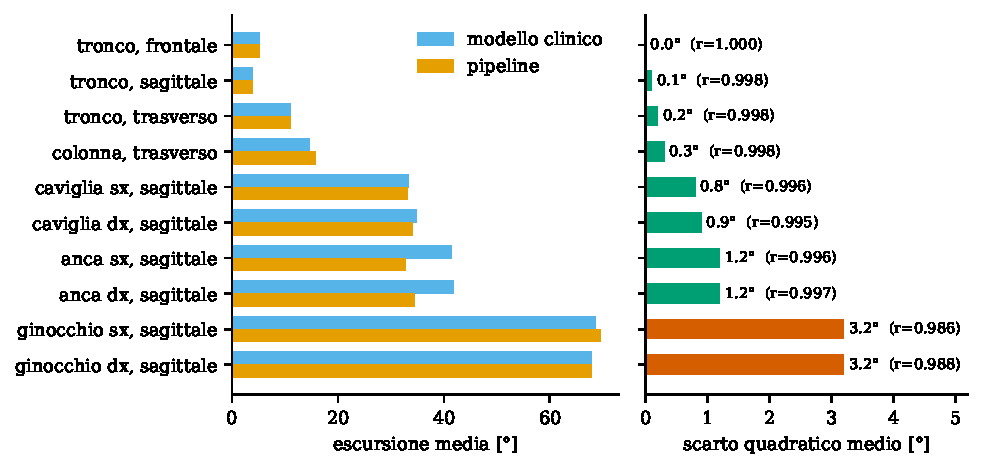
\includegraphics[width=\textwidth]{figures/appendice/app_validazione.pdf}
\caption{Validazione per giunto su 118 prove. A sinistra l'escursione media
secondo il modello clinico e secondo la pipeline; a destra lo scarto quadratico
medio sulla serie temporale, con la correlazione.}
\label{fig:app:validazione}
\end{figure}



%   ACKNOWLEDGEMENTS
\cleardoublepage
\pagenumbering{gobble}
\thispagestyle{plain}			% Supress header
\section*{Ringraziamenti}
% TODO: scrivere i ringraziamenti.

\vspace{1.5cm}
\hfill
Claudio Rocchetti, L'Aquila, % TODO: mese e anno

\newpage				% Create empty back of side
\thispagestyle{empty}
\mbox{}


\end{document} 
